\documentclass[12pt, a4paper]{article}
\usepackage[utf8]{inputenc}
% \usepackage[russian]{babel}
\usepackage[pdftex]{graphicx, color}
\usepackage{amsmath, amsfonts, amssymb, amsthm}
\usepackage{bm}
\usepackage[left=2cm,right=2cm,top=1.5cm,bottom=2cm]{geometry}
\usepackage{indentfirst}
\usepackage{hyperref}
\usepackage{textcomp}
\usepackage{float}

\usepackage[table,xcdraw]{xcolor}
\usepackage{diagbox}
\usepackage{tikz}
\usetikzlibrary{tikzmark}

\graphicspath{{pics/}}

\begin{document}
    \begin{center}
        
\includegraphics[height=3cm]{UVM.png}

        {\large\textbf{
            CS253A QR: Reinforcement Learning: Assignment \textnumero 2
        }}

        \vspace{0.3cm}

        \textit{\textbf{Ayat Ospanov}}

        \today
    \end{center}

    \tableofcontents
    \section{2.1}\label{sec:2.1}
        If $\varepsilon = 0.5$, each second step is the greedy step. This means the probability
        of choosing the greedy action is at least $0.5$. Further, as we do random step with the
        probability of $0.5$ and select greedy action in this step with the probability of $\frac{1}{2}$
        (because we have two actions and one of them is the greedy action), the probability of
        randomly selecting the greedy action is $0.25$. Therefore, the overall probability of
        selecting the greedy action is $0.75$.

        We can generalize this task to the case of $n$ options/actions and any $\varepsilon$. The answer
        is $(1 - \varepsilon) + \frac{\varepsilon}{n}$.

    \section{2.2}
        \begin{table}[H]
            \centering
            \caption{Work of a bandit algorithm}
            \label{tab:algo}
            \begin{tabular}{|l|l|l|l|l|l|}
                \hline
                \rowcolor[HTML]{C0C0C0}
                \backslashbox{}{t} & \multicolumn{1}{c|}{\cellcolor[HTML]{C0C0C0}1} & \multicolumn{1}{c|}{\cellcolor[HTML]{C0C0C0}2} & \multicolumn{1}{c|}{\cellcolor[HTML]{C0C0C0}3} & \multicolumn{1}{c|}{\cellcolor[HTML]{C0C0C0}4} & \multicolumn{1}{c|}{\cellcolor[HTML]{C0C0C0}5} \\ \hline
                $A_i$ & 1\tikzmark{a1} & 2\tikzmark{a2} & 2\tikzmark{a3} & 2\tikzmark{a4} & 3\tikzmark{a5} \\
                $R_i$ & -1 & 1 & -2 & 2 & 0 \\ \hline
                $Q_i(1)$ & 0\tikzmark{q1} & -1 & -1 & -1 & -1 \\
                $Q_i(2)$ & 0 & 0\tikzmark{q2} & 1\tikzmark{q3} & -0.5\tikzmark{q4} & 0.(3) \\
                $Q_i(3)$ & 0 & 0 & 0 & 0 & 0\tikzmark{q5} \\
                $Q_i(4)$ & 0 & 0 & 0 & 0 & 0 \\ \hline
                Choice & Random & Random & Greedy & $\varepsilon$ case & Random \\ \hline
            \end{tabular}
        \end{table}

        \begin{tikzpicture}[overlay, remember picture]
            \draw [->, thick] ({pic cs:q1}) [bend right] to ({pic cs:a1});
            \draw [->, thick] ({pic cs:q2}) [bend right] to ({pic cs:a2});
            \draw [->, thick] ({pic cs:q3}) [bend right] to ({pic cs:a3});
            \draw [->, thick] ({pic cs:q4}) [bend right] to ({pic cs:a4});
            \draw [->, thick] ({pic cs:q5}) [bend right] to ({pic cs:a5});
        \end{tikzpicture}

        On the table \ref{tab:algo} the work of a bandit algorithm is provided by time step.
        Each arrow shows the Q-value of a chosen action. As on greedy step an algorithm
        choose the $\text{arg}\max_a Q_t(a)$, the only case of choosing the argmax is
        step 3. On the step 4 the algorithm chose the value of $-0.5$ which is not the
        argmax. It means that at this step the $\varepsilon$ case has occured. On the
        other steps (1, 2, 5) as we have more that one maximum value of Q, the alogrithm
        chose random argmax. On these steps $\varepsilon$ case could possibly have occurred.

    \section{2.3}
        In the long run, $\varepsilon = 0.01$ will act better as 99.1\% of the time (see Section.
        \ref{sec:2.1}) it choose the correct actions, while in the case of $\varepsilon = 0.1$
        the rate of correct actions is $0.91 \text{ or } 91\%$.

    \section{2.4}
        \begin{align*}
            Q_{n+1} &= (1 - \alpha_n)Q_n + \alpha_n R_n =\\
                    &= (1 - \alpha_n) [(1 - \alpha_{n-1})Q_{n-1} + \alpha_{n-1}R_{n-1}] + \alpha_n R_n =\\
                    &= (1 - \alpha_n) (1 - \alpha_{n-1}) Q_{n-1} + \alpha_{n-1}(1 - \alpha_n) R_{n-1} + \alpha_n R_n =\\
                    &=\prod_{i=1}^n(1-\alpha_i)Q_1 + \sum_{i=1}^n\Big(\alpha_i \prod_{j=i+1}^n(1-\alpha_j)R_i\Big)
        \end{align*}

    \section{2.5}
        Orange lines -- constant learning rate (step-size)

        Blue lines -- step-size = $\frac{1}{n}$

        \begin{figure}[H]
            \centering
            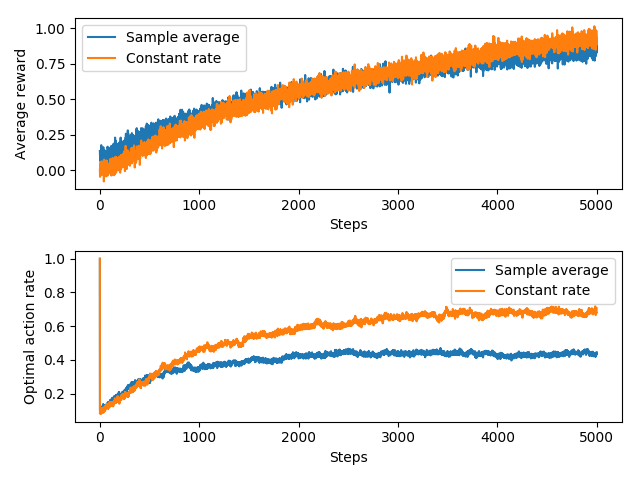
\includegraphics[width=0.8\linewidth]{1.png}
            \caption{Initial values for $q_*(a)$ are equal}
        \end{figure}

        \begin{figure}[H]
            \centering
            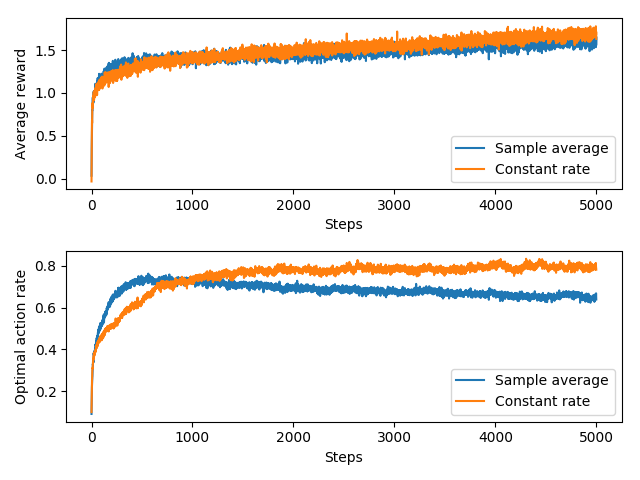
\includegraphics[width=0.8\linewidth]{2.png}
            \caption{Initial values for $q_*(a)$ are randomly sampled from normal distribution}
        \end{figure}

        When initial values for $q_*(a)$ are equal, the convergence is slow. Also in this case the rate of optimal solutions is 1 in the beginning because all values are equal and therefore optimal. When initial values for $q_*(a)$ are random, convergence is faster. In both cases algorithm with a constant step-size converges faster. Moreover, in the case of random $q_*(a)$ sample average method decreases in rate of optimal actions, because it doesn't adapt to the new rewards. Thus, we were convinced that constant step-size is better for nonstationary problems.





\end{document}
